\documentclass{beamer}
%%%%%%%%%%%%%%%%%%%%%%%%%%%%%%%  Packages  %%%%%%%%%%%%%
\usepackage{amsmath} 
\usepackage{mathtools}
\usepackage{physics}
\usepackage{amssymb}
\usepackage{mathptmx}
\usepackage{array}
  
\usepackage[sort&compress]{natbib}     % bib

%%%%%%%%% FIGurES %%%%%%%%%%%%%%%%%%%%%%%%
\usepackage{textcomp}
\usepackage{graphicx}
\usepackage{caption} 
\usepackage{subcaption}
\usepackage{scrextend}
\usepackage{rotating}
\usepackage{float}
\usepackage{hyperref}

\usepackage{multimedia}

%\graphicspath{{./figures/}}
\hypersetup{colorlinks=true, citecolor=blue, linkcolor=blue}
\renewcommand{\equationautorefname}{Eq.}
\renewcommand{\figureautorefname}{Fig.}
 
%%%%%%%%%%%% LaNgUaGe %%%%%%%%%%%%%%%%%%
\usepackage{verbatim}
\usepackage{natbib}
\usepackage{wrapfig}
\usepackage[utf8]{inputenc}

%%%%%%%%%%%%%% PhYsIcS %%%%%%%%%%%%%%%%%%%%%%%

\renewcommand{\annia}{\hat{a}}
\renewcommand{\annib}{\hat{b}}
\renewcommand{\creata}{\hat{a}^\dagger}
\renewcommand{\creatb}{\hat{b}^\dagger}

\renewcommand{\a}{a^ }
\renewcommand{\b}{b^ }
\renewcommand{\adag}{a^\dagger}
\renewcommand{\bdag}{b^\dagger}

\usepackage{qcircuit}



%%%%%%%%%%%%%%%%%5 TIKZ %%%%%%%%%%%%%%%%%%%%

\usepackage{tikz}
\usetikzlibrary{positioning,calc}

%\tikzset{>=stealth}

%\newcommand{\tikzmark}[1]{\tikz[baseline,remember picture] \node[anchor=base, #1] (#1) {};}
%\newcommand{\tikzmark}[3][]{\tikz[overlay,remember picture,baseline] \node [anchor=base,#1](#2) {#3};}
\newcommand{\tikzmark}[3][]{\tikz[remember picture,baseline] \node [anchor=base,#1](#2) {$#3$};}
\usetheme{PaloAlto}

\title{Modelling Nonlinear optics with the Bloch-Messiah reduction}
\author{Oliver Thomas, Dara McCutcheon, Will McCutcheon}
\institute{Quantum Engineering CDT \\ University of Bristol}
\date{\today}

% plan

\begin{document}

% slide 1
\frame{\titlepage}

% slide 2
\begin{frame}
\frametitle{Overview}
\begin{itemize}
	\item What is nonlinear optics?
    \item Why do we care about it?
    \item What I have been doing
    \item Gaussian optics 
    \item Outlook
\end{itemize}
\end{frame}

%slide 3
\begin{frame}
\frametitle{Motivation quantum nonlinear optics}
\begin{columns}
\column{0.5\textwidth}
    \begin{block}{The good}
    Spontaneous Parametric processes, SPDC, SFWM
    \begin{itemize}
        \item Heralded single photon sources
        \item Entangled photon pair generation (polarisation, spatial)
    \end{itemize}
    Kerr processes 
    \begin{itemize}
        \item Self-Phase modulation (SPM), generating Bannana states (CV)
        \item Cross-Phase modulation (XPM) for sensing
    \end{itemize}
    \end{block}
%
\column{0.5\textwidth}
    \begin{block}{The bad}
        Spontaneous parametric processes
        \begin{itemize}
            \item Generating more than two photons -$>$ bad for quantum computing
            \item Understanding filtering
        \end{itemize}
        All Kerr nonlinear processes 
        \begin{itemize}
            \item SPM -$>$ Spectral broadening
            \item XPM -$>$ Unwanted phase shifts on single photons due to propagation of the pump 
        \end{itemize}
        \end{block}
\end{columns}

\end{frame}

% slide 4
\begin{frame}
\frametitle{What do we mean by nonlinear optics?}
\begin{itemize} 
    \item Roughly processes that conserve energy but do not conserve photon number. 
        \begin{equation}
            \vec{P}= \chi^{(1)} \vec{E_1} + \chi^{(2)}\vec{E_1}\vec{E_2} + \chi^{(3)}\vec{E_1}\vec{E_2}\vec{E_3} + \dots
        \end{equation}
\end{itemize}
Here we are going to talk about squeezing, i.e SPDC or SFWM, Hamiltonians are then of the form, 
\begin{equation} 
    \hat{H} = A \creata_S \creata_I \annia_P + h.c.
\end{equation}
\begin{equation} 
    \hat{H} = A \creata_S \creata_I \annia_P \annia_P + h.c.
\end{equation}
%\textbf{Note} for the rest of this presentation I will drop the hat notatiaion and using the convention a, b are annihilation operators in modes a \& b
\end{frame}

%slide 9
\begin{frame}
\frametitle{Gaussian Optics}

    \begin{itemize}
    \item Using the undelpeted pump approximation we can write the Hamiltonians as terms which are at most quadratic in creation and annihilation operators. 
\end{itemize}
        \begin{equation}
        \hat{U} = \exp[-\frac{i}{\hbar}\left( \tikzmark{P}{P} \int d\omega_1 \int d\omega_2 \tikzmark{f}{f(\omega_1,\omega_2)} \tikzmark{aa}{ \creata_s(\omega_1) \creata_i(\omega_2)} + h.c. \right) ]
    \end{equation}

    \begin{tikzpicture}[overlay, remember picture, node distance=1cm]
    
    \node[red] (power) [below =of P]{Power};
    \draw[red,->,thick] (power) to [in=-90,out=45] (P);
    
    \node[blue,xshift=0cm] (jsa) [below =of f]{JSA};
    \draw[blue,->,thick] (jsa) to [in=-90,out=135] (f.south);
    
    \node[purple] (sigidler) [below =of aa]{Signal \& Idler};
    \draw[purple,->,thick] (sigidler) to [in=-90,out=45] (aa.south);
\end{tikzpicture}
\vspace{10pt} 
\begin{itemize}
    \item These are Gaussian transforms, they take Gaussian states to Gaussian states \footnote{These are linear symplectic transforms which conviently can be written as a matrix}

\end{itemize}

    \begin{equation}
    \begin{bmatrix} 
        \vec{\b}   \\
        \vec{\bdag}
    \end{bmatrix}
    = 
    \textbf{M}
    \begin{bmatrix}
        \vec{\a} \\
        \vec{\adag}
    \end{bmatrix}
\end{equation}

\end{frame}

% slide 10
\begin{frame}
\frametitle{Types of Gaussian transformations}
%
\begin{figure}[h]
\begin{align*}
\centering
    \Qcircuit @C=0.6cm @R=0.2cm{
    %1
        &\lstick{a_1} &\qw &\multigate{1}{Squeezer} &\qw &\qw &\measureD{} \\
    %2
        &\lstick{a_2} &\qw &\ghost{Squeezer} &\qw  &\multigate{1}{BS} &\measureD{} \\
    %3
        &\lstick{a_3} &\qw &\multigate{1}{Squeezer} &\qw &\ghost{BS} &\measureD{} \\
    %4
        &\lstick{a_4} &\qw &\ghost{Squeezer} &\qw &\qw &\measureD{} \\
}
\end{align*}
\caption{Two source HOM dip}
\end{figure}
%
    \vspace{-20pt}
% 
\begin{figure}[h]
\begin{align*}
\centering
    \Qcircuit @C=0.5cm @R=0.2cm{
    %1
        &\lstick{a_1} &\qw &\multigate{1}{Squeezer} &\qw &\qw &\measureD{} & \\
    %2
        &\lstick{a_2} &\qw &\ghost{Squeezer} &\qw  &\multigate{1}{PBS} &\gate{\pi/4} &\measureD{H \& V} \\
    %3
        &\lstick{a_3} &\qw &\multigate{1}{Squeezer} &\qw &\ghost{PBS} &\measureD{} \\
    %4
        &\lstick{a_4} &\qw &\ghost{Squeezer} &\qw &\qw &\measureD{} \\
}
\end{align*}
\caption{Type-1 Fusion gate}
\end{figure}
%
\end{frame}


    % slide 
\begin{frame}{Reducing the size of the state-space}
    We can re-write the Hamiltonian using a Schmidt-decomposition as,
    \begin{equation}
    P' F(\omega_1,\omega_2) = \sum_k r_k \psi_k(\omega_1) \phi_k(\omega_2)
    \end{equation}

    Where $r_k$ is the Schmidt number, $ \psi $ \& $\phi $ are unitaries.\newline

    To solve this numerically we discretize the function and the Schmidt-decomposition is then the Singular value decomposition (SVD) of the JSA (F).
    \begin{equation}
        P' \textbf{F}_{(\omega_1, \omega_2)} = \sum_k r_k \textbf{U}_{(\omega_1, k)} \textbf{V}_{(k, \omega_2)}^\dagger
    \end{equation}
    \begin{itemize}
        \item with $ \psi_k(\omega_1) $ is the k-th row and $\omega_1$-th column of $\textbf{U}_{(\omega_1, k)}$,
        \item with $ \phi_k(\omega_2) $ is the $\omega_2$-th row and k-th column of $\textbf{V}^\dagger_{(k,\omega_2)}$
    \end{itemize}
\end{frame}

%slide 7
\begin{frame}{Joint Spectral Amplitudes (JSAs)} 
    \centering
        \begin{figure}
            \movie[height=0.65\textwidth,width=1\textwidth, loop, autostart]{}{jsasepgauss.mp4}
        \end{figure}
        \footnotetext{Moving to the rotating frame...}
    \end{frame}

% slide 
    \begin{frame}{Seperable JSAs Schmidt modes}
        
    \begin{figure}
        \centering
    \begin{subfigure}{0.4\textwidth}
        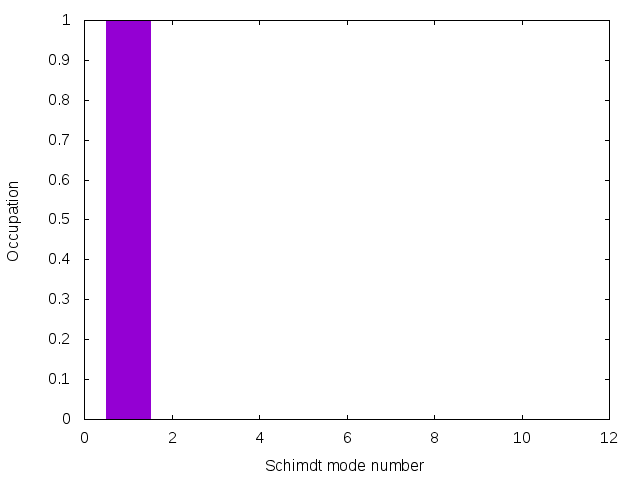
\includegraphics[width=1\textwidth]{sepschmidtmodesocc.png}
    \end{subfigure}
    ~
    \begin{subfigure}{0.5\textwidth}
        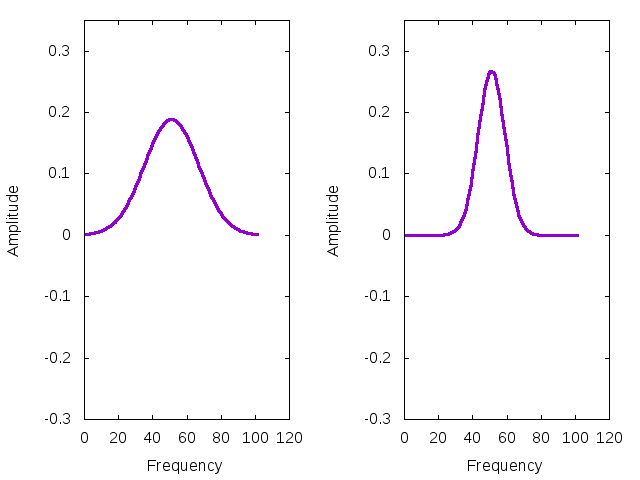
\includegraphics[width=1\textwidth]{sepsingle_sig_idler1.png}
        \caption{Signal (red) and Idler (blue)}
        \end{subfigure}
    \end{figure}

\end{frame} 

%slide 8
\begin{frame}{Non-separable JSAs} 
    \begin{figure}
        \centering
            \movie[height=0.65\textwidth,width=1\textwidth, loop, autostart]{}{jsanotsepsincgauss.mp4}
        \end{figure}
    \end{frame}
%
    \begin{frame}{Non-separable JSAs Schimdt modes}
    \begin{figure}
        \centering
        \begin{subfigure}{0.4\textwidth}
            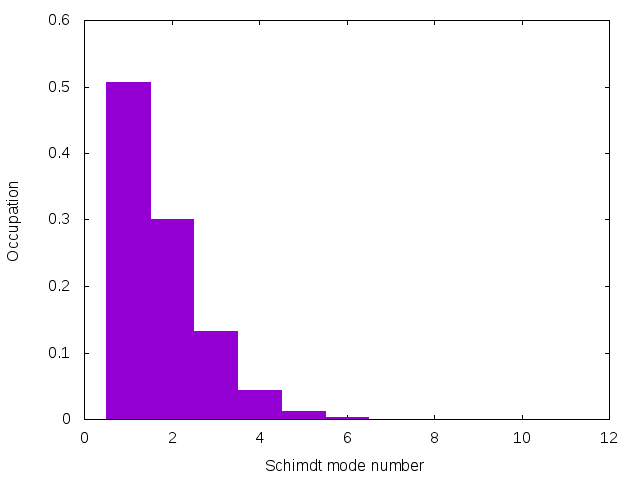
\includegraphics[width=1\textwidth]{notsepschmidtmodesocc.png}
        \end{subfigure}
        ~
        \begin{subfigure}{0.5\textwidth}
        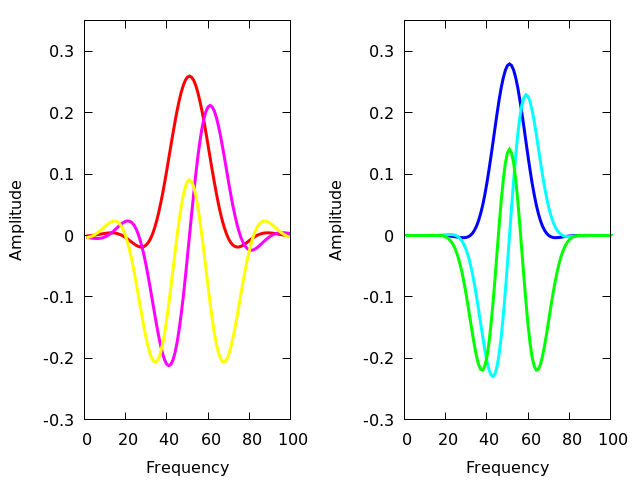
\includegraphics[width=1\textwidth]{notsepsingle_sig_idler1.png}
        \caption{Signal (red) and Idler (blue)}
        \end{subfigure}
    \end{figure}

\end{frame} 

%slide 11
\begin{frame}{Two squeezers JSA} 
    \begin{figure}
        \centering
        \begin{subfigure}{0.45\textwidth}
       \movie[height=0.9\textwidth, width=1\textwidth, loop, autostart]{}{jsa12pickme.mp4}
        \end{subfigure}
        ~
        \begin{subfigure}{0.45\textwidth}
        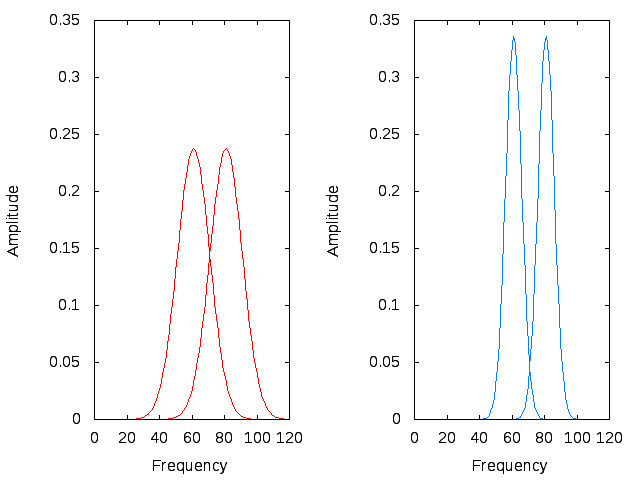
\includegraphics[width=1\textwidth]{single_sig_idler12.png}
    \end{subfigure}
   \end{figure}

\end{frame} 

% slide 10
\begin{frame}
\frametitle{Correlations in a HOM dip}
%

\begin{figure}[h]
\begin{align*}
\centering
    \Qcircuit @C=0.6cm @R=0.2cm{
    %1
        &\lstick{a_1} &\qw &\multigate{1}{Squeezer} &\qw &\qw &\measureD{} \\
    %2
        &\lstick{a_2} &\qw &\ghost{Squeezer} &\qw  &\multigate{1}{BS} &\measureD{} \\
    %3
        &\lstick{a_3} &\qw &\multigate{1}{Squeezer} &\qw &\ghost{BS} &\measureD{} \\
    %4
        &\lstick{a_4} &\qw &\ghost{Squeezer} &\qw &\qw &\measureD{} \\
}
\end{align*}
\caption{Two source HOM dip}
\end{figure}
\end{frame}
% slide 12
\begin{frame}
    \frametitle{G(4) correlation function}
    \begin{equation}
        G^{(4)} = \frac{ \left< \creata_1 \creata_2 \creata_3 \creata_4 \annia_1 \annia_2 \annia_3 \annia_4 \right>}
        {\left< \creata_1 \annia_1 \right> \left< \creata_2 \annia_2 \right> \left< \creata_3 \annia_3 \right> \left< \creata_4 \annia_4 \right>}
    \end{equation}
    Where,
    \begin{equation}
        a_i = \sum_j a_{i}(\omega_j)
    \end{equation}
    Meaning we sum over all of the spectral modes of the spatial modes (1,2,3,4) seperately.
    We end up with, 
    \begin{equation}
        G^{(4)} = 1 - \left( \frac{2 \mid cosh(r) \mid^2}{\mid cosh(r) \mid ^2 + \mid sinh(r) \mid^2} sin(\theta) cos(\theta) \right)^2
    \end{equation}
\end{frame}

\begin{frame}{G(4) correlation function}

    \begin{figure}[h]
       \movie[height=0.7\textwidth, width=1\textwidth, loop, autostart]{}{g4python.mp4}
    \end{figure}
\end{frame}

%slide 13
\begin{frame}
\frametitle{Summary}
\begin{itemize}
\end{itemize}
\end{frame}


%slide 13
\begin{frame}
\frametitle{Outlook}
\begin{itemize}
\end{itemize}
\end{frame}

\bibliographystyle{unsrt}
\bibliography{refs}
\end{document}
